% higgs_composite_qg.tex (generated; edit src/higgs_composite_qg.template.tex) -- Regular Article for Physical Review D (REVTeX 4.2).
% PROJECT spacetimes, folder Revision_HS_CJT_and_Kohn-Sham/paper_prd.
% This file is generated from src/higgs_composite_qg.template.tex by scripts/build_paper.py, which inserts every number
% that a program computes, from the data files and the reports of the checks of the folder data/ (the bounds of the
% agreement of two computations rounded up).  Typed in the template are only the parameters of the model and of the
% numerical method, mathematical constants, and measured values of the Standard Model and of cosmology with their references.
% Build:  python3 scripts/build_paper.py   (writes higgs_composite_qg.tex and runs pdflatex and bibtex)
\documentclass[aps,prd,twocolumn,superscriptaddress,nofootinbib,floatfix,longbibliography]{revtex4-2}
\usepackage{amsmath,amssymb}
\usepackage{graphicx}
\usepackage{bm}
\usepackage[colorlinks=true,linkcolor=blue,citecolor=blue,urlcolor=blue]{hyperref}
\hypersetup{pdftitle={Higgs as a Composite, and Quantum Gravity},pdfauthor={Patrick Lee Nash}}

% the suffixes of the symbols of PROJECT spacetimes: LL (the Lorentz super-loop, Ref. [Nash2026]) and SF (the superfluid)
\newcommand{\LL}{{\rm LL}}
\newcommand{\SF}{{\rm SF}}
\newcommand{\tr}{\mathrm{tr}}

\begin{document}

\title{Higgs as a Composite, and Quantum Gravity}

\author{Patrick Lee Nash, Ph.D.}
\affiliation{PROJECT spacetimes}

\date{November 21, 2026}

\begin{abstract}
The unit bi-octonions form a Moufang loop, the Lorentz super-loop, that contains $SL(2,\mathbb C)$ and eight spinor
charges; these are carried by a Dirac isodoublet on Minkowski space, coupled to the gauge group
$SL(2,\mathbb C)\times SU(2)_{\rm v}\times U(1)^{\rm F}$ of the local Lorentz transformations, the isospin and the fermion
number. With a contact self-interaction whose spin-zero pair channel is supercritical, the spinor field condenses into a
superfluid whose order parameter is a composite isospin vector of fermion number two. We solve it in five mean-field
methods (Hubbard-Stratonovich with three decouplings, Kohn-Sham, and Cornwall-Jackiw-Tomboulis) and derive its effective
Lagrangians. In every method the condensate realizes the Higgs mechanism: the isospin bosons $W^\pm$ and the
fermion-number boson $Z$ become massive, exactly one gauge boson (the photon) stays massless, and the surviving group is
$SL(2,\mathbb C)\times O(2)$, whose identity component contains the $U(1)$ of the electric charge. The amplitude mode is a
composite scalar bound below the threshold of two quasi-particles. From the static pair response we compute the gradient
coefficient of the order parameter at the critical temperature and find Ginzburg numbers 7.6\mbox{--}11: the critical region
is wider than the critical temperature itself, and the mean-field transition is not reliable. Against the Standard Model, the amplitude mode is
8.8\mbox{--}11 times too heavy relative to the scale of the breaking ($M_H/v=4.46\mbox{--}5.69$ against $0.5085$), strongly coupled,
broad ($\Gamma_H/M_H\approx2.1\mbox{--}3.9$ at tree level), and accompanied by charged scalars of about the same mass.
The Higgs boson of this model is therefore composite by construction, but it is not the boson observed at the LHC. We
outline how gravitation enters through E.~A.~Lord's gauge theory of the local change of spinor representation, for which
the $SL(2,\mathbb C)$ factor of the gauge group is the natural place; the gravitational sector is not computed here.
\end{abstract}

\maketitle

%=====================================================================================================================
\section{Introduction}
\label{sec:intro}

The particle discovered at the Large Hadron Collider in 2012~\cite{ATLAS2012,CMS2012} has, within uncertainties of a few
per cent, the couplings of the elementary Higgs boson of the Standard Model~\cite{ATLAS2022,CMS2022,PDG2024}. Whether the
Higgs field is elementary or a composite of more fundamental fields is nevertheless one of the oldest open questions about
it. Composite proposals range from technicolor~\cite{Weinberg1976,Susskind1979} and the condensation of the top
quark~\cite{Miransky1989,BHL1990} to a Higgs boson that is a pseudo-Goldstone boson of a strongly coupled
sector~\cite{KaplanGeorgi1984,Agashe2005}; the review of Hill and Simmons~\cite{HillSimmons2003} describes the dynamics. Their
common prototype is the model of Nambu and Jona-Lasinio~\cite{NJL1961}: a four-fermion interaction above a critical
strength condenses the fermion field, the fermions acquire a gap, and a composite scalar appears whose mass is tied to
that gap.

In earlier work~\cite{Nash2026} the author showed that the unit bi-octonions form a Moufang loop, the Lorentz super-loop,
that contains $SL(2,\mathbb C)$ together with eight spinor charges, a Weyl spinor that is an isospin doublet, and that a
spin-zero superfluid of these charges forms isospin-triplet pairs. The present paper asks whether such a superfluid can
be the Higgs sector of a gauge theory: whether it gives masses to gauge bosons while leaving a massless photon, whether
its amplitude mode can be the Higgs particle, and whether the Higgs is then a composite particle. We set up the gauge
theory of the spinor field (Sec.~\ref{sec:model}), solve its superfluid in five mean-field methods
(Sec.~\ref{sec:methods}), derive the effective Lagrangians, the collective modes, the masses of the gauge bosons and the
surviving symmetry (Sec.~\ref{sec:T0}), compute the free energy at finite temperature and the Ginzburg number of the
transition (Sec.~\ref{sec:thermal}), compare the result with the Higgs sector of the Standard Model
(Sec.~\ref{sec:higgs}), and discuss compositeness (Sec.~\ref{sec:composite}).

The answers are as follows. In every method the superfluid realizes the Higgs mechanism, with a massless photon; its
amplitude mode is a composite scalar below the threshold of two quasi-particles; and the Higgs field of the model is
composite by construction. But the amplitude mode is 8.8\mbox{--}11 times too heavy against the scale of the breaking, broad,
and strongly coupled, the thermal transition lies deep in its own critical region, and there are charged scalars that the
Standard Model does not have: this composite Higgs is not the observed boson.

The gauge group of the model contains $SL(2,\mathbb C)$ as a gauge factor with a Lorentz connection, which is a pure gauge
on the flat space-time of this paper. E.~A.~Lord~\cite{Lord1971} showed that the local change of representation of the
two-component spinor algebra, made a Yang-Mills gauge group, leads with the necessary auxiliary fields to a self-interacting
spin-two field identical with Einstein's gravitation. Section~\ref{sec:gravity} outlines how that construction will
make the gravitational sector of the present model; it is a program, and no part of it is computed here. Every number of
this paper is produced by two independent programs (Rust and Python), and the statements of Secs.~\ref{sec:methods} to
\ref{sec:higgs}, except the mass matrix of the gauge bosons and the time-dependent calculations, are checked a third time by
a notebook in the Wolfram Language; the Supplemental Material~\cite{SM} gives the derivations, the checks and the data.

%=====================================================================================================================
\section{The model}
\label{sec:model}

\paragraph*{Space-time and spinor field.}
Space-time is the manifold M31 of the Hermitian bi-quaternions, which is Minkowski space with the metric
$\eta^\LL={\rm diag}(1,-1,-1,-1)$~\cite{Nash2026}; we use $\hbar=c=k_{\rm B}=1$. The spinor charges of the super-loop are
carried by a Dirac isodoublet $\Psi_\LL$ with eight complex components (four Dirac components times two isospin components)
and the mass $m_\LL=0.2$. The momenta of the uniform states are restricted to $|\vec q_\LL|<\Lambda_\LL=1$; the cutoff
$\Lambda_\LL$ is the unit of energy throughout.

\paragraph*{Gauge group and covariant derivative.}
The group of the local transformations is
\begin{equation}
\mathrm{GEE}=SL(2,\mathbb C)\times SU(2)_{\rm v}\times U(1)^{\rm F}_\LL ,
\label{eq:GEE}
\end{equation}
the local Lorentz transformations of the spinor index, the isospin (vector-like: it acts on both chiralities alike) and
the fermion number $F_\LL$. The covariant derivative of the spinor field is
\begin{equation}
\nabla_p\Psi_\LL=\big(\partial_p+\Gamma^\LL_p+ig^{\rm v}_\LL\mathsf W_{\SF,p}+ig^{\rm F}_\LL B_{\SF,p}\big)\Psi_\LL ,
\label{eq:cov}
\end{equation}
with the Lorentz (spin) connection $\Gamma^\LL_p$, the isospin gauge field
$\mathsf W_{\SF,p}=\sum_{\iota=1}^3W^\iota_{\SF,p}\,\tau^\LL_\iota/2$ with the coupling
$g^{\rm v}_\LL=0.7$ (the Pauli matrices $\tau^\LL_\iota$ act on the isospin index), and the gauge field $B_{\SF,p}$ of the
fermion number with $g^{\rm F}_\LL=0.45$. On flat M31 the connection $\Gamma^\LL_p$ is a pure gauge and is set to zero.

\paragraph*{Lagrangian.}
The Lagrangian is
\begin{multline}
\mathcal L_\SF=\bar\Psi_\LL\Big(i\sum_p\gamma^p_\LL\nabla_p-m_\LL\Big)\Psi_\LL\\
-\tfrac14\sum_\iota W^\iota_{\SF,pp'}W^{\iota,pp'}_\SF-\tfrac14B_{\SF,pp'}B^{pp'}_\SF-V^{(2)}_\SF ,
\label{eq:L}
\end{multline}
with the field strengths of $W$ and $B$ and the contact self-interaction
\begin{multline}
V^{(2)}_\SF=\tfrac12G^{\rm S}_\SF{:}(\bar\Psi_\LL\Psi_\LL)^2{:}+\tfrac12G^{\rm V}_\SF\sum_p\eta^\LL_{pp}{:}(j^{{\rm F},p}_\SF)^2{:}\\
-\tfrac14G_\LL\sum_{\iota=1}^3{:}(\Pi^\iota_\LL)^\dagger\Pi^\iota_\LL{:}
\label{eq:V2}
\end{multline}
($G^{\rm S}_\SF=2.8$, $G^{\rm V}_\SF=0.8$, $G_\LL=25.2$; colons denote normal order with respect to the filled Dirac sea),
where $j^{{\rm F},p}_\SF=\bar\Psi_\LL\gamma^p_\LL\Psi_\LL$ is the fermion-number current and
\begin{equation}
\Pi^\iota_\LL=\Psi_\LL^T\mathsf K^\iota_\LL\Psi_\LL,\qquad\mathsf K^\iota_\LL=(\mathsf C_\LL\gamma^{\rm ch}_\LL)\otimes(\mathsf E_\LL\tau^\LL_\iota)
\label{eq:pairs}
\end{equation}
are the pair operators of the spin-zero, isospin-one channel (Lorentz scalar, fermion number 2), with the
charge-conjugation matrix $\mathsf C_\LL$, the chirality matrix $\gamma^{\rm ch}_\LL$ and $\mathsf E_\LL=i\tau^\LL_2$. The
potential (\ref{eq:V2}) is the second step of a recursion~\cite{SM}: the author's first potential, a scalar attraction and a
vector repulsion, admits no superfluid in any method; adding the pairing term makes the methods that keep the exchange
contraction (Kohn-Sham and CJT) condense in the scalar channel instead; (\ref{eq:V2}) keeps the effective scalar coupling of
the first potential and the effective pair coupling of the second, and admits a superfluid in all methods.

\paragraph*{The composite field.}
The model has no elementary scalar field. The field of the superfluid is the complex isospin vector
$\vec\Phi^X_\SF=(\Phi^{X,1}_\SF,\Phi^{X,2}_\SF,\Phi^{X,3}_\SF)$ of the amplitudes of the pair self-energy that a method $X$
assigns to a state,
\begin{equation}
\mathsf P_\SF=\sum_{\iota=1}^3\Phi^{X,\iota}_\SF(\mathsf K^\iota_\LL)^\dagger ,
\label{eq:Phi}
\end{equation}
a composite of two spinor charges with the covariant derivative
$\nabla_p\vec\Phi=\partial_p\vec\Phi+2ig^{\rm F}_\LL B_{\SF,p}\vec\Phi-g^{\rm v}_\LL\vec W_{\SF,p}\times\vec\Phi$ of an isospin
vector of fermion number 2.

%=====================================================================================================================
\section{Five mean-field methods}
\label{sec:methods}

A uniform quasi-free state is described, at every momentum, by its normal and pair correlation matrices; it is the
thermal state of the Bogoliubov-de Gennes matrix
\begin{equation}
\mathsf H_\SF(\vec q_\LL)=\begin{pmatrix}\mathsf h_\LL(\vec q_\LL)+\mathsf N_\SF&\mathsf P_\SF\\\mathsf P_\SF^\dagger&-\big(\mathsf h_\LL(-\vec q_\LL)+\mathsf N_\SF\big)^T\end{pmatrix},
\label{eq:BdG}
\end{equation}
with the free matrix $\mathsf h_\LL(\vec q)=(\vec\alpha_\LL\cdot\vec q+\beta_\LL m_\LL)\otimes\mathsf 1_2$ and the normal and
pair self-energies $\mathsf N_\SF$, $\mathsf P_\SF$, the derivatives of the energy per volume with respect to the
correlations. The energy of the contact terms is evaluated with Wick's theorem; its direct (Hartree), exchange (Fock) and
pair (Bogoliubov) contractions are kept with weights that define the methods:
\begin{itemize}
\item HS $(s_{\rm S},s_{\rm V})$: Hubbard-Stratonovich~\cite{Hubbard1959,Stratonovich1957} at the saddle point, with the
shares $s_{\rm S}$, $s_{\rm V}$ of the scalar and vector terms decoupled in the density channel and the rest in the pair
channel; we compute $(s_{\rm S},s_{\rm V})=(1,1)$, $(0,1)$, $(0,0)$;
\item KS: the method of Kohn and Sham~\cite{HohenbergKohn1964,KohnSham1965,Mermin1965}, with the exchange contraction in
the local-density approximation of the densities $n$ and $n_{\rm S}$;
\item CJT: the two-particle-irreducible effective action of Cornwall, Jackiw and Tomboulis~\cite{CJT1974} truncated at the
contractions of the contact terms (all three kept).
\end{itemize}
Each method has an effective coupling $g^{X,{\rm S}}_\SF$ in the scalar density channel and $g^{X,{\rm P}}_\SF$ in the pair
channel $\mathsf K^3_\LL$ (Table~\ref{tab:T0}). The pair channel of the normal state is unstable when
\begin{equation}
\lambda^{\rm P}_\SF(T)=\frac{g^{X,{\rm P}}_\SF\,I_1\big(M^{X,{\rm n}}_\SF(T),T\big)}{\pi^2}>1,
\label{eq:lambda}
\end{equation}
with $I_1(M,T)=\int_0^{\Lambda_\LL}q^2\tanh(E/2T)\,E^{-1}dq$, $E=(q^2+M^2)^{1/2}$, and the Dirac mass $M^{X,{\rm n}}_\SF(T)$ of
the normal state. All five methods have
$\lambda^{\rm P}_\SF(0)>1$ (Table~\ref{tab:T0}); in the methods with $g^{X,{\rm S}}_\SF\neq0$ the scalar density shifts the
Dirac mass.

The uniform states are computed on a grid of 24 Gauss-Legendre momenta on $[0,\Lambda_\LL]$ times six directions (exact
for the uniform states, whose correlations depend on the direction only through angular momenta 0 and 1, and at second
order in the twists of Sec.~\ref{sec:thermal}),
self-consistent to $10^{-12}$ or better, by a Rust program and, independently, by a Python program (numpy and LAPACK); a
notebook in the Wolfram Language repeats the checks with a third implementation~\cite{SM}. Time-dependent calculations use the
integrators CVODE and IDA of SUNDIALS~\cite{SUNDIALS2005,SUNDIALS2022}. Every number of this paper is an output of these
programs~\cite{SM,Repo}.

%=====================================================================================================================
\section{The superfluid at zero temperature}
\label{sec:T0}

\paragraph*{Ground state and gap.}
In every method the ground state is a polar superfluid, $\vec\Phi^X_\SF=\Phi^X_{0,\SF}e^{i\vartheta}\vec n$ with a real unit
vector $\vec n$, whose quasi-particles have the energies $\pm E(\vec q)=\pm(q^2+(M^{X,{\rm D}}_\SF)^2+(\Phi^X_{0,\SF})^2)^{1/2}$
(eight times each). The pair amplitude acts as a gap added in quadrature to the Dirac mass $M^{X,{\rm D}}_\SF$ of the
superfluid; the gap is $E^{X,{\rm gap}}_\SF=((M^{X,{\rm D}}_\SF)^2+(\Phi^X_{0,\SF})^2)^{1/2}$. Table~\ref{tab:T0} lists the
numbers.

\begin{table*}
\caption{\label{tab:T0}The five methods with the potential (\ref{eq:V2}): effective couplings, the eigenvalue
(\ref{eq:lambda}) of the pair response of the normal vacuum, the superfluid at $T=0$ (order parameter, Dirac mass, gap,
depth of the effective potential below the normal vacuum) and the critical temperature (Sec.~\ref{sec:thermal}), in
units of $\Lambda_\LL$.}
\begin{ruledtabular}
\begin{tabular}{lddddddddd}
method & \multicolumn{1}{c}{$g^{X,{\rm S}}_\SF$} & \multicolumn{1}{c}{$g^{X,{\rm P}}_\SF$} & \multicolumn{1}{c}{$\lambda^{\rm P}_\SF(0)$} & \multicolumn{1}{c}{$\Phi^X_{0,\SF}$} & \multicolumn{1}{c}{$M^{X,{\rm D}}_\SF$} & \multicolumn{1}{c}{$E^{X,{\rm gap}}_\SF$} & \multicolumn{1}{c}{$10^4|\mathcal V^X_\SF(\Phi_0)|$} & \multicolumn{1}{c}{$T^{X,{\rm c}}_\SF$} & \multicolumn{1}{c}{$E^{X,{\rm gap}}_\SF/T^{X,{\rm c}}_\SF$} \\
\hline
HS (1,1) & 2.80 & 25.2 & 1.1838 & 0.40306 & 0.20669 & 0.45297 & 5.186 & 0.26047 & 1.739 \\
HS (0,1) & 0 & 24.5 & 1.1510 & 0.36201 & 0.20000 & 0.41358 & 3.608 & 0.24047 & 1.720 \\
HS (0,0) & 0 & 23.7 & 1.1134 & 0.30699 & 0.20000 & 0.36639 & 2.062 & 0.21380 & 1.714 \\
KS & -7.40 & 23.7 & 1.1134 & 0.32849 & 0.16229 & 0.36639 & 2.422 & 0.22212 & 1.650 \\
CJT & -7.40 & 23.7 & 1.1134 & 0.32849 & 0.16229 & 0.36639 & 2.422 & 0.22212 & 1.650 \\
\end{tabular}
\end{ruledtabular}
\end{table*}

\paragraph*{Effective Lagrangians.}
The effective potential $\mathcal V^X_\SF(\vec\Phi)$ is the smallest energy per volume of method $X$ among the uniform
states with the field $\vec\Phi$, measured from the normal vacuum; it is computed point by point with an applied pair field
and a self-consistent normal self-energy~\cite{SM}. It has the form of a Mexican hat (Fig.~\ref{fig:potential}); a Landau
polynomial $a|\vec\Phi|^2+b|\vec\Phi|^4+c|\vec\Phi|^6$ fits it to 0.27\mbox{--}0.70\% of its depth, but no polynomial is exact:
the series of $\mathcal V^X_\SF$ in $|\vec\Phi|^2$ about the origin has a radius of convergence of the order of $m_\LL$, smaller
than the order parameter~\cite{SM}. The
kinetic part allowed by GEE has two invariants,
\begin{equation}
\mathcal L^X_{\rm kin}=\sum_p\eta^\LL_{pp}\Big[Z^X_\SF(\nabla_p\vec\Phi)^\dagger\cdot\nabla_p\vec\Phi+Y^X_\SF\frac{|\vec\Phi^\dagger\cdot\nabla_p\vec\Phi|^2}{|\vec\Phi|^2}\Big],
\label{eq:Lkin}
\end{equation}
whose coefficients follow from the static susceptibilities $\chi^{ab}_\SF$ of the vacuum to the chemical potentials of the
isospin and of the fermion number: $Z^X_\SF=\chi^{11}_\SF/(2\Phi_0^2)$ and $Z^X_\SF+Y^X_\SF=\chi^{\rm FF}_\SF/(8\Phi_0^2)$. With the
Yang-Mills terms, $\mathcal L^X=\mathcal L^X_{\rm kin}-\mathcal V^X_\SF+\mathcal L^{\rm YM}$ is the Lagrangian of a complex isospin
vector of fermion number 2 with a Mexican-hat potential: the structure of the Higgs sector of the Standard Model, with an
isospin vector in place of the doublet. The decay constants of the Goldstone fields of the phase and of the isospin
rotations are $f^{X,{\rm F}}_\SF=(2(Z^X_\SF+Y^X_\SF))^{1/2}\Phi^X_{0,\SF}$ and $f^{X,{\rm I}}_\SF=(2Z^X_\SF)^{1/2}\Phi^X_{0,\SF}$.

\begin{figure}
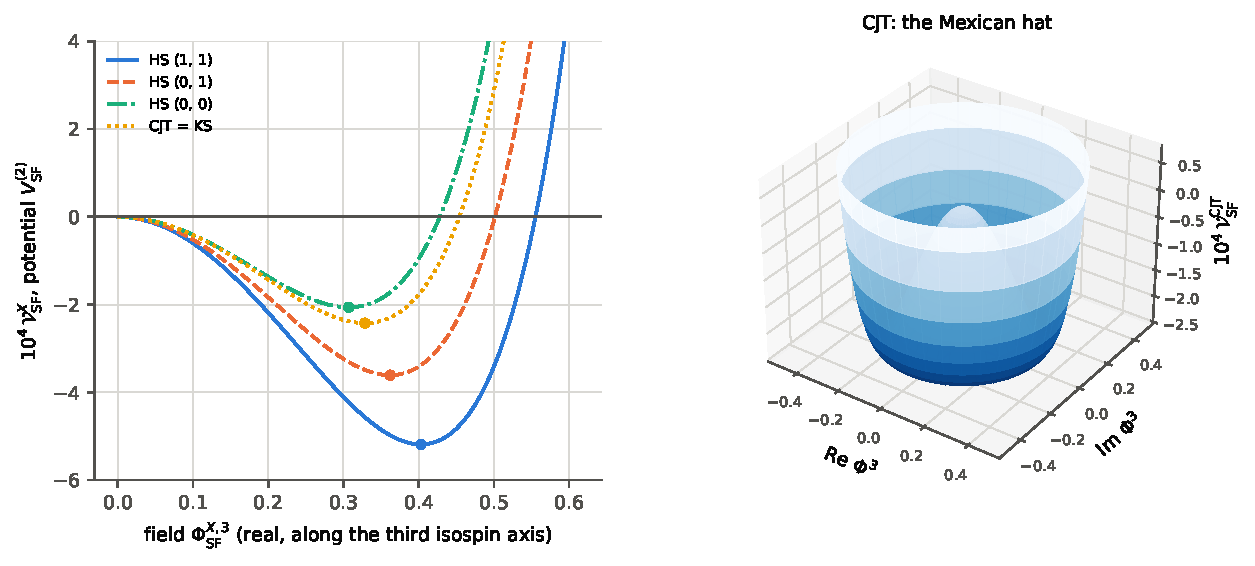
\includegraphics[width=\columnwidth]{fig_part3_q1_potential.pdf}
\caption{\label{fig:potential}Left: the effective potentials $\mathcal V^X_\SF$ along a polar direction of the field for
the five methods (KS and CJT coincide along the polar fields). Right: the Mexican hat of CJT over the complex plane of
$\Phi^{\rm CJT,3}_\SF$. Units of $\Lambda_\LL$.}
\end{figure}

\paragraph*{Collective modes.}
The linear response of the vacuum (the small oscillations of each method, without any expansion in derivatives) has, for
the polar vacuum along $\vec e_3$, an amplitude (Higgs) mode $h^X_\SF$ of charge 0 and a doublet of non-unitary modes of
charge $\pm1$ (the imaginary parts of the components 1 and 2 relative to the phase), with the masses
$M^{X,{\rm H}}_\SF$ and $M^{X,{\rm NU}}_\SF$ of Table~\ref{tab:higgs}; both lie below the threshold $2E^{X,{\rm gap}}_\SF$ of two
quasi-particles, at 0.82\mbox{--}0.90 of it for the amplitude mode. The three Goldstone fields (the phase and two isospin
angles) are massless without the gauge fields.

\paragraph*{Gauge bosons, photon and surviving group.}
Inserting a constant field into (\ref{eq:Lkin}) gives the mass matrix of the four gauge fields
$(W^1,W^2,W^3,B)$. For a polar vacuum $\vec\Phi=\Phi_0e^{i\vartheta}\vec n$ it is diagonal in a frame adapted to $\vec n$, with the
eigenvalues $0$ (the field $\vec n\cdot\vec W$), $(M^X_{W,\SF})^2$ twice and $(M^X_{Z,\SF})^2$,
\begin{equation}
M^X_{W,\SF}=g^{\rm v}_\LL f^{X,{\rm I}}_\SF ,\qquad M^X_{Z,\SF}=2g^{\rm F}_\LL f^{X,{\rm F}}_\SF ,
\label{eq:masses}
\end{equation}
and the same masses follow from the microscopic response of the superfluid to constant gauge fields, to
$3\times10^{-12}$ of $(M^X_{Z,\SF})^2$~\cite{SM}. The massless gauge bosons correspond one to one to the generators that leave the field
unchanged (a theorem that holds for every field, because the mass matrix is positive semidefinite~\cite{SM}): for a polar
vacuum the only such generator is $\vec n\cdot\vec T$, so the photon is $A=\vec n\cdot\vec W$; it does not mix with $B$ (the
weak mixing angle vanishes) because the condensate has fermion number 2, so no admixture of $F_\LL$ leaves it unchanged. For
a field with a mixed stabilizer the massless boson does mix (Fig.~\ref{fig:mixing}), with $\tan\theta'=g^{\rm v}_\LL/(2g^{\rm F}_\LL)$,
the analogue of the Weinberg angle with $g'$ replaced by $2g^{\rm F}_\LL$. The surviving group of the vacuum along $\vec e_3$ is
$SL(2,\mathbb C)\times O(2)$: the identity component of $O(2)$ is the group $U(1)^{\rm Q}_\LL$ of the electric charge
$Q_\LL=T^3_\LL$ (charges $\pm\frac12$ of the spinor field, $\pm1$ of $W^\pm$), and its second component is a charge conjugation
of the photon. Of the fourteen degrees of freedom (four massless vector fields and the six real components of $\vec\Phi$),
the three Goldstone fields become the longitudinal parts of $W^\pm$ and $Z$; a time-dependent calculation in the temporal
and in the unitary gauge (CVODE and IDA) shows the Goldstone wave of the phase turning into the longitudinal $Z$ with the
dispersion $\omega^2=k^2+M_Z^2$~\cite{SM}. The $SL(2,\mathbb C)$ factor is unbroken: the condensate is a Lorentz scalar.

\begin{figure}
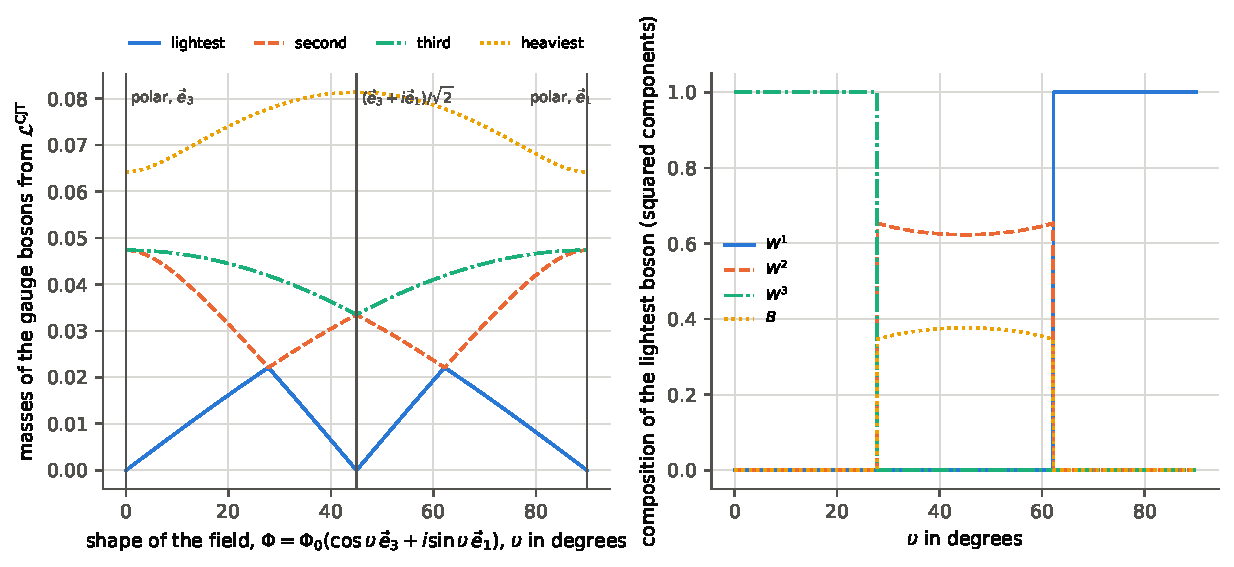
\includegraphics[width=\columnwidth]{fig_part4_r1_massmatrix.pdf}
\caption{\label{fig:mixing}The mass matrix of the effective Lagrangian of CJT along the fields
$\Phi_0(\cos\upsilon\,\vec e_3+i\sin\upsilon\,\vec e_1)$. Left: the four masses. Right: the composition of the lightest boson. A
massless boson exists only where the field has a continuous stabilizer ($\upsilon=0$, $45^\circ$, $90^\circ$); at
$\upsilon=45^\circ$ it is $\cos\theta'W^2-\sin\theta'B$ with $\theta'=37.875^\circ$.}
\end{figure}

%=====================================================================================================================
\section{Finite temperature and the width of the critical region}
\label{sec:thermal}

\paragraph*{Free energy and critical temperature.}
At the temperature $T$ the uniform state is the thermal state $f(\mathsf H_\SF)$ of (\ref{eq:BdG}), with the Fermi function
$f$, and its free energy per volume is $\mathcal E^X_\SF-T\mathcal S_\SF$ with the energy of method $X$ and the entropy of
the quasi-free state (for HS the saddle point at finite $T$, for CJT the truncated effective action at finite
$T$~\cite{AmelinoCamelia1993}, for KS Mermin's functional~\cite{Mermin1965} with the exchange-correlation energy of $T=0$).
The critical temperature solves $\lambda^{\rm P}_\SF(T)=1$ in (\ref{eq:lambda}); it is unique because $\lambda^{\rm P}_\SF$ does not
increase with $T$ (checked on a fine grid of temperatures). Table~\ref{tab:T0} gives $T^{X,{\rm c}}_\SF=0.214\mbox{--}0.260$ and
$E^{X,{\rm gap}}_\SF(0)/T^{X,{\rm c}}_\SF=1.65\mbox{--}1.74$, of the size of the ratio $1.764$ of the theory of Bardeen, Cooper and
Schrieffer~\cite{BCS1957}. The gap equation $1=g^{X,{\rm P}}_\SF I_1(E^{X,{\rm gap}}_\SF,T)/\pi^2$ fixes the gap at every
temperature, and since the scalar density of the superfluid contains the same integral, the Dirac mass of the superfluid
does not depend on the temperature~\cite{SM}. The order parameter changes by less than 0.14\% up to $0.3\,T^{X,{\rm c}}_\SF$ and
vanishes like $(1-T/T^{X,{\rm c}}_\SF)^{1/2}$ at $T^{X,{\rm c}}_\SF$ (Fig.~\ref{fig:thermal}); near $T^{X,{\rm c}}_\SF$ it lies inside the radius of
convergence of the series of the free energy in $|\vec\Phi|^2$, and the mean-field free energy takes the form of Landau's
theory.

\begin{figure*}
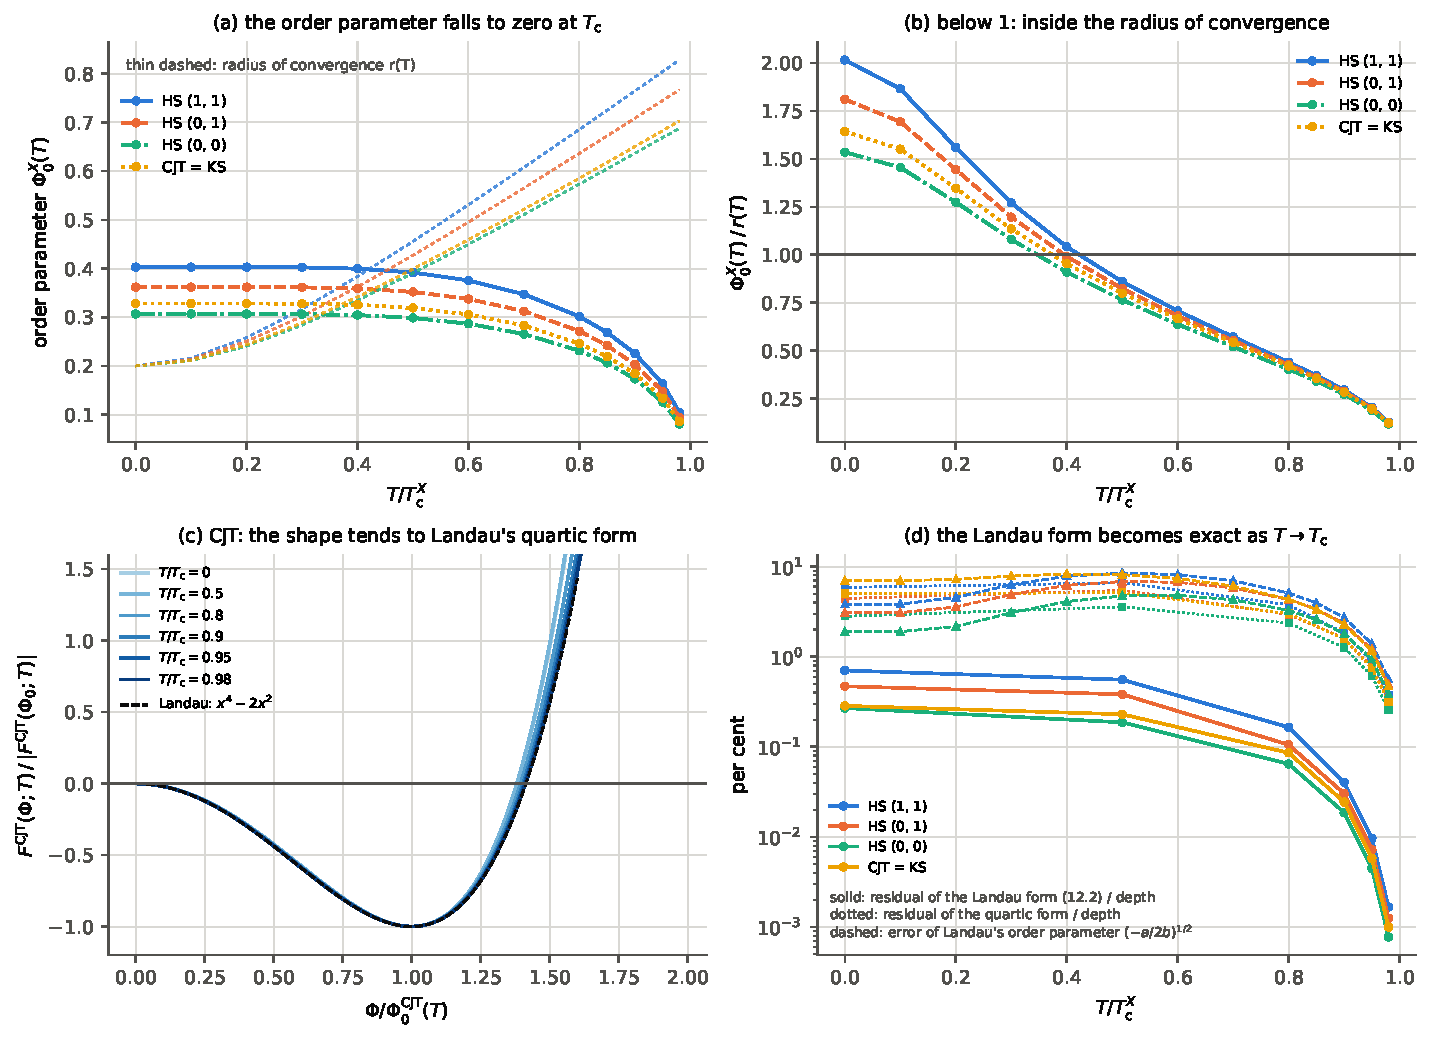
\includegraphics[width=0.85\textwidth]{fig_part3_q4_thermal.pdf}
\caption{\label{fig:thermal}The mean-field free energy at finite temperature. (a) The order parameter against
$T/T^{X,{\rm c}}_\SF$ (KS and CJT coincide), with the radius of convergence $(M^{X,{\rm n}}_\SF(T)^2+\pi^2T^2)^{1/2}$ of the series of
the free energy in $|\vec\Phi|^2$ (thin dashed). (b) Their ratio. (c) The free energy of CJT, normalized to its depth, with the
curve $x^4-2x^2$ of Landau's theory (dashed). (d) The residuals of the sextic (``Landau form'') and of the quartic fit, and
the error of the order parameter $(-a/2b)^{1/2}$ of Landau's theory. The mean field is not reliable near $T^{X,{\rm c}}_\SF$
(Sec.~\ref{sec:thermal}).}
\end{figure*}

\paragraph*{Ginzburg-Landau functional.}
The fluctuations of the order parameter, which no mean-field method contains, decide whether this behaviour is real.
Near $T^{X,{\rm c}}_\SF$ a static field that varies slowly in space has the free energy
\begin{equation}
\mathcal F^{X,{\rm GL}}_\SF=\int d^3x\Big[\mathsf c^X_\SF\sum_{j=1}^3|\partial_j\vec\Phi|^2+\alpha^{X,{\rm GL}}_\SF t\,|\vec\Phi|^2+b^X_\SF|\vec\Phi|^4\Big],
\label{eq:GL}
\end{equation}
with $t=(T-T^{X,{\rm c}}_\SF)/T^{X,{\rm c}}_\SF$; rotations, isospin rotations and the conservation of fermion number allow no other
term of second order, and the two quartic invariants $|\vec\Phi|^4$ and $|\vec\Phi\cdot\vec\Phi|^2$ coincide on the polar fields.
The slope $\alpha^{X,{\rm GL}}_\SF$ and the quartic coefficient $b^X_\SF$ follow from the free energy of uniform fields; the
gradient coefficient $\mathsf c^X_\SF$ needs a field that varies in space.

\paragraph*{The gradient coefficient.}
A pair field moving with the momentum $q$ along $\vec e_3$ has the coefficient of $|\vec\Phi|^2$
$a(q;T)=a(0;T)+\mathsf c^X_\SF q^2+O(q^4)$. Its state pairs the momenta $\vec q_\LL\pm\frac12q\vec e_3$; after the gauge transformation
$\Psi\to e^{iqx^3/2}\Psi$ it is the thermal state of (\ref{eq:BdG}) with $\mathsf h_\LL(\pm\vec q_\LL)$ replaced by
$\mathsf h_\LL(\pm\vec q_\LL)+\frac12q\,\alpha^3_\LL\otimes\mathsf 1_2$, the normal self-energy of the normal state (a change of
it affects the free energy only at fourth order in the field), and a small pair block $\mathsf P^{\rm a}_\SF$. Its pair matrix,
summed over the momenta, is the static pair response
\begin{equation}
\mathsf C^{\rm p,tot}_\SF=-\int\frac{d^3q_\LL}{(2\pi)^3}\sum_{a,b=1}^8\frac{f(\varepsilon^{\rm A}_a)-f(\varepsilon^{\rm D}_b)}{\varepsilon^{\rm A}_a-\varepsilon^{\rm D}_b}\,\mathsf u_a\mathsf u_a^\dagger\mathsf P^{\rm a}_\SF\mathsf w_b\mathsf w_b^\dagger ,
\label{eq:chi}
\end{equation}
with the eigenvalues and eigenvectors $(\varepsilon^{\rm A}_a,\mathsf u_a)$ of the particle block and
$(\varepsilon^{\rm D}_b,\mathsf w_b)$ of the hole block of the twisted matrix, and its free energy, from the normal state, is to
second order
\begin{equation}
\mathcal F^X_2=\tfrac12\,{\rm Re}\,\tr\Big[\big(\mathsf P^{\rm a}_\SF-\mathsf P^X_\SF[\mathsf C^{\rm p,tot}_\SF]\big)\big(\mathsf C^{\rm p,tot}_\SF\big)^\dagger\Big],
\label{eq:F2}
\end{equation}
where $\mathsf P^X_\SF[\cdot]$ is the pair self-energy of method $X$ (all of its pair channels). The free energy of the field is
the minimum of (\ref{eq:F2}) at fixed $\Phi^{X,3}_\SF=\tr(\mathsf K^3_\LL\mathsf P^X_\SF)/8$: the components of $\mathsf P^{\rm a}_\SF$ along
the three $(\mathsf K^\iota_\LL)^\dagger$ are held fixed and the 25 others are made self-consistent. Then
$a(q;T)=\mathcal F^X_2/|\Phi^{X,3}_\SF|^2$, and at $q=0$
\begin{equation}
a(0;T)=\frac{1-\lambda^{\rm P}_\SF(T)}{\lambda^{\rm P}_\SF(T)\,g^{X,{\rm P}}_\SF},\qquad\alpha^{X,{\rm GL}}_\SF=-\frac{T^{X,{\rm c}}_\SF}{g^{X,{\rm P}}_\SF}\,\frac{d\lambda^{\rm P}_\SF}{dT}\Big|_{T^{X,{\rm c}}_\SF},
\label{eq:a0}
\end{equation}
which the three implementations confirm to $2\times10^{-11}$~\cite{SM}. The cutoff must be placed on the relative momentum $\vec q_\LL$ of the pair:
with a cutoff on the momenta of the two charges, $|\vec q_\LL\pm\frac12q\vec e_3|<\Lambda_\LL$, a moving pair loses the pairs in a
shell of thickness $\propto|q|$ at the cutoff, and $a(q;T)-a(0;T)$ becomes linear in $|q|$ (Fig.~\ref{fig:ginzburg}a): the
gradient expansion does not exist. Two quantities measure the remaining error of the regularization: the twist of the
unbroken generator $T^3_\LL$, which should cost nothing, costs 18\mbox{--}21\% of $\mathsf c^X_\SF$; and nonlinear twisted
states with a self-consistent normal self-energy, whose spurious current feeds back through the vector interaction, give
values that differ by 10\mbox{--}11\% (and by $-$60\% in CJT)~\cite{SM}.

\paragraph*{The Ginzburg number.}
Above $T^{X,{\rm c}}_\SF$ the $n=6$ real components of $\vec\Phi$ fluctuate with the weight $\exp(-\mathcal F^{X,{\rm GL}}_\SF/T)$; to
Gaussian order their free energy per volume is $\frac n2T\int\frac{d^3k}{(2\pi)^3}\ln(\mathsf c k^2+\alpha t)$, whose specific
heat $n\alpha^{3/2}/(16\pi\mathsf c^{3/2}t^{1/2})$ diverges at $T^{X,{\rm c}}_\SF$. The specific heat of the mean-field theory
(\ref{eq:GL}) jumps by $\Delta C=\alpha^2/(2bT^{X,{\rm c}}_\SF)$. The two are equal at the Ginzburg
number~\cite{Levanyuk1959,Ginzburg1960}
\begin{equation}
{\rm Gi}^X_\SF=\frac{n^2b^2(T^{X,{\rm c}}_\SF)^2}{64\pi^2\,\alpha\,\mathsf c^3}=\frac{n^2}{256\pi^2\,(\Delta C\,\xi^3)^2},
\label{eq:Gi}
\end{equation}
with the correlation length $\xi=(\mathsf c/\alpha)^{1/2}$ of the mean-field theory at $|t|=1$, and mean-field theory requires $|t|\gg{\rm Gi}^X_\SF$; the second form shows that it needs many degrees of freedom,
$\Delta C\,\xi^3\gg1$, in a correlation volume. (Other forms of the criterion change the numerical factor, not the
combination.) Table~\ref{tab:gi} and Fig.~\ref{fig:ginzburg} give the result:
${\rm Gi}^X_\SF=7.6\mbox{--}11$. The critical region is wider than $T^{X,{\rm c}}_\SF$ itself: even at $|t|=1$ the Gaussian
fluctuations alone exceed the mean-field jump, $C^{\rm fl}/\Delta C=({\rm Gi}^X_\SF)^{1/2}=2.8\mbox{--}3.4$. The cause is
visible in the numbers: the correlation length $\xi=1.05\mbox{--}1.35$ is about the cutoff length (the pairs are tightly bound:
there is no Fermi surface, and the coupling is above the critical one), and a correlation volume holds
$\Delta C\,\xi^3=0.035\mbox{--}0.043$ degrees of freedom. A superconductor of the theory of Bardeen, Cooper and Schrieffer, with a
coherence length much larger than the distance between electrons, is the opposite case. Within the error of the
regularization, ${\rm Gi}^X_\SF$ lies between 4.6 and 23.

\begin{table}
\caption{\label{tab:gi}The coefficients of (\ref{eq:GL}) at $T^{X,{\rm c}}_\SF$, the correlation length $\xi$ (units
$1/\Lambda_\LL$), the specific-heat jump per correlation volume, and the Ginzburg number (\ref{eq:Gi}). KS and CJT have the same
normal state and pair channels at $T^{X,{\rm c}}_\SF$.}
\begin{ruledtabular}
\begin{tabular}{lcccccc}
method & $10^2\alpha$ & $10^2b$ & $10^2\mathsf c$ & $\xi$ & $\Delta C\xi^3$ & ${\rm Gi}$ \\
\hline
HS (1,1) & 1.4038 & 1.2389 & 1.5487 & 1.050 & 0.0354 & 11.4 \\
HS (0,1) & 1.2699 & 1.3764 & 1.7138 & 1.162 & 0.0382 & 9.77 \\
HS (0,0) & 1.0743 & 1.5943 & 1.9528 & 1.348 & 0.0415 & 8.28 \\
KS & 1.1176 & 1.4724 & 1.9272 & 1.313 & 0.0432 & 7.62 \\
CJT & 1.1176 & 1.4724 & 1.9272 & 1.313 & 0.0432 & 7.62 \\
\end{tabular}
\end{ruledtabular}
\end{table}

\begin{figure*}
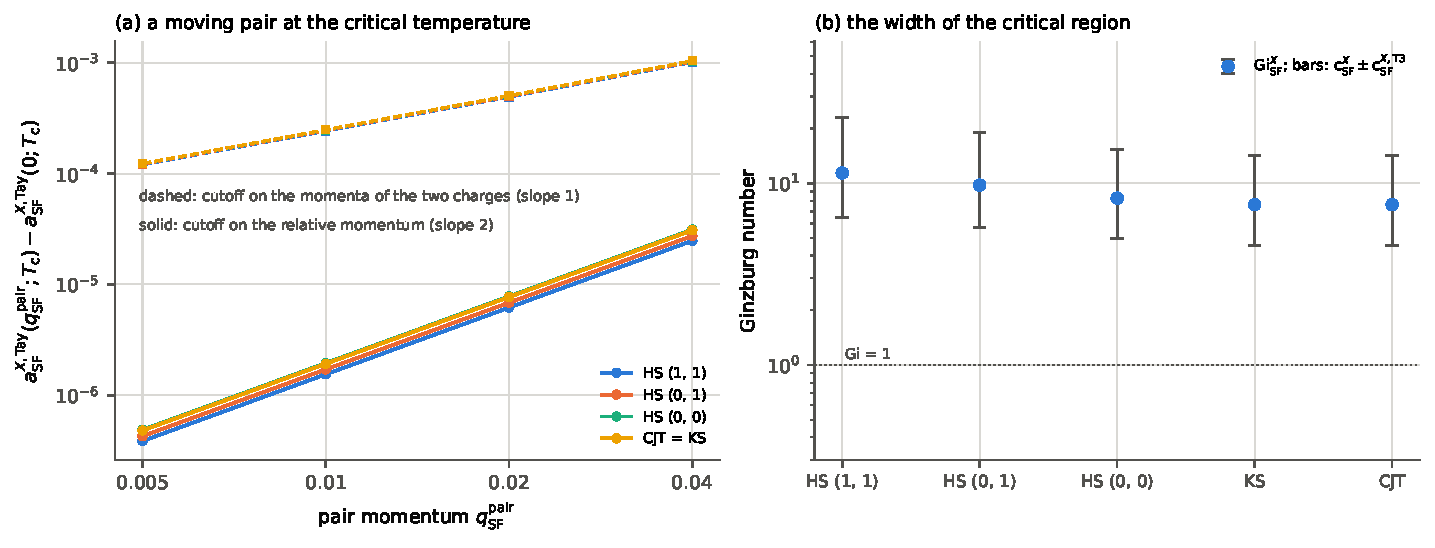
\includegraphics[width=0.85\textwidth]{fig_prd_ginzburg.pdf}
\caption{\label{fig:ginzburg}(a) $a(q;T^{X,{\rm c}}_\SF)-a(0;T^{X,{\rm c}}_\SF)$ against the momentum $q$ of the pair: quadratic for
the cutoff on the relative momentum (solid), linear for the cutoff on the momenta of the two charges (dashed). (b) The
Ginzburg number (\ref{eq:Gi}) of the five methods; the bars show the range for $\mathsf c^X_\SF$ changed by the spurious
coefficient of the $T^3_\LL$ twist.}
\end{figure*}

The statements of mean-field theory near $T^{X,{\rm c}}_\SF$ (the critical temperature, the exponent $\frac12$, the continuity of
the transition) therefore do not describe the model; the agreement of the five methods there is no evidence, because all
of them omit the same fluctuations. For a field with two quartic invariants the fluctuations may even make the transition
discontinuous~\cite{PelissettoVicari2002}, and gauge fields can do the same~\cite{HLM1974}; in the electroweak theory the
thermal transition ends at a critical Higgs mass, above which it is a crossover~\cite{Kajantie1996,DOnofrio2016}. A
reliable answer needs the three-dimensional theory (\ref{eq:GL}) with gauge fields on a lattice, or the Gaussian fluctuations
of the pair field~\cite{NozieresSchmittRink1985}.

%=====================================================================================================================
\section{Can the superfluid play the role of the Higgs particle?}
\label{sec:higgs}

In the Standard Model $M_W=gv/2$ with $v=(\sqrt2G_F)^{-1/2}=246.22$~GeV, $m_H=125.20\pm0.11$~GeV, and the Higgs boson is
narrow, $\Gamma_H=3.7^{+1.9}_{-1.4}$~MeV~\cite{PDG2024,CMSwidth2022}. By (\ref{eq:masses}) the analogue of $v$ is
\begin{equation}
v^X_\SF=2f^{X,{\rm I}}_\SF ,\qquad M^X_{W,\SF}=\tfrac12g^{\rm v}_\LL v^X_\SF ,
\label{eq:vSF}
\end{equation}
independent of the gauge coupling, and the natural dimensionless numbers are $M^{X,{\rm H}}_\SF/v^X_\SF$ (Standard Model
$0.5085$) and the quartic coupling $\lambda^{X,{\rm H}}_\SF=(M^{X,{\rm H}}_\SF)^2/(2(v^X_\SF)^2)$ (Standard Model $0.1293$).

\paragraph*{Width.}
The kinetic part (\ref{eq:Lkin}), with $\vec\Phi=(\Phi_0+h/(2(Z+Y))^{1/2})e^{i\vartheta_0}R_1(\vartheta_1)\vec e_3$, contains the
couplings $f^{X,{\rm F}}_\SF h(\partial\vartheta_0)^2$ and $((f^{X,{\rm I}}_\SF)^2/f^{X,{\rm F}}_\SF)h(\partial\vartheta_{1,2})^2$: for the
canonically normalized Goldstone fields all three are $1/f^{X,{\rm F}}_\SF$. The decay of $h$ into two massless Goldstone
quanta then has the width $(M^{X,{\rm H}}_\SF)^3/(32\pi(f^{X,{\rm F}}_\SF)^2)$ in each channel, and
\begin{equation}
\Gamma^{X,{\rm H}}_\SF=\frac{3\,(M^{X,{\rm H}}_\SF)^3}{32\pi\,(f^{X,{\rm F}}_\SF)^2},
\label{eq:width}
\end{equation}
which by the equivalence theorem~\cite{CLT1974,ChanowitzGaillard1985} is also the width into $W^+W^-$ and $ZZ$, up to corrections
of relative order $x=M_V^2/(M^{X,{\rm H}}_\SF)^2$, where $M_V$ is the mass of $W$ or $Z$: here $M_V\le0.11\,M^{X,{\rm H}}_\SF$, and
the tree-level factor $(1-4x)^{1/2}(1-4x+12x^2)$ of these channels lowers the width by less than 7\%. For $f=v$,
(\ref{eq:width}) is the width $3m_H^3/(32\pi v^2)$ of a heavy Standard-Model Higgs boson. The effective Lagrangian is used at the energy $M^{X,{\rm H}}_\SF$, where it is not accurate (its own mass of the
amplitude mode differs from the linear response by 7.0\mbox{--}17\%), so (\ref{eq:width}) gives the order of magnitude.

\begin{table*}
\caption{\label{tab:higgs}The superfluid as a Higgs sector. Masses in units of $\Lambda_\LL$ (gauge boson masses at
$g^{\rm v}_\LL=0.7$, $g^{\rm F}_\LL=0.45$); the last rows set $v^X_\SF=246.22$~GeV. The last column gives the Standard
Model~\cite{PDG2024}; its thermal crossover is at $159.5\pm1.5$~GeV~\cite{DOnofrio2016} and has no critical region.}
\begin{ruledtabular}
\begin{tabular}{lcccccc}
quantity & HS (1,1) & HS (0,1) & HS (0,0) & KS & CJT & Standard Model \\
\hline
$v^X_\SF=2f^{X,{\rm I}}_\SF$ & 0.1431 & 0.1354 & 0.1228 & 0.1314 & 0.1353 & 246.22 GeV \\
$f^{X,{\rm F}}_\SF$ & 0.07097 & 0.06723 & 0.06139 & 0.07135 & 0.07135 & -- \\
$M^{X,{\rm H}}_\SF$ (amplitude mode) & 0.8137 & 0.7251 & 0.6144 & 0.6035 & 0.6035 & 125.20 GeV \\
$M^{X,{\rm NU}}_\SF$ (charged scalars) & 0.8061 & 0.7251 & 0.6144 & 0.6573 & 0.6440 & -- \\
$M^X_{W,\SF}$ & 0.0501 & 0.0474 & 0.0430 & 0.0460 & 0.0474 & 80.37 GeV \\
$M^X_{Z,\SF}$ & 0.0639 & 0.0605 & 0.0553 & 0.0642 & 0.0642 & 91.19 GeV \\
$M^{X,{\rm H}}_\SF/v^X_\SF$ & 5.69 & 5.35 & 5.00 & 4.59 & 4.46 & 0.5085 \\
$\lambda^{X,{\rm H}}_\SF$ & 16.2 & 14.3 & 12.5 & 10.5 & 9.94 & 0.1293 \\
$M^{X,{\rm H}}_\SF/M^X_{W,\SF}$ & 16.2 & 15.3 & 14.3 & 13.1 & 12.7 & 1.558 \\
$M^X_{W,\SF}/M^X_{Z,\SF}$ & 0.784 & 0.783 & 0.778 & 0.716 & 0.738 & 0.8814 \\
$M^{X,{\rm H}}_\SF/2E^{X,{\rm gap}}_\SF$ & 0.898 & 0.877 & 0.838 & 0.824 & 0.824 & -- \\
$M^{X,{\rm NU}}_\SF/M^{X,{\rm H}}_\SF$ & 0.991 & 1.00 & 1.00 & 1.09 & 1.07 & none \\
$f^{X,{\rm F}}_\SF/f^{X,{\rm I}}_\SF$ & 0.992 & 0.993 & 1.00 & 1.09 & 1.05 & -- \\
$\Gamma^{X,{\rm H}}_\SF/M^{X,{\rm H}}_\SF$, Eq.~(\ref{eq:width}) & 3.9 & 3.5 & 3.0 & 2.1 & 2.1 & $3\times10^{-5}$ \\
$T^{X,{\rm c}}_\SF/v^X_\SF$ & 1.82 & 1.78 & 1.74 & 1.69 & 1.64 & 0.648 \\
$\Lambda_\LL$ [GeV] & 1721 & 1818 & 2005 & 1874 & 1820 & -- \\
$M^{X,{\rm H}}_\SF$ [GeV] & 1400 & 1318 & 1232 & 1131 & 1098 & 125.20 \\
$T^{X,{\rm c}}_\SF$ [GeV] & 448 & 437 & 429 & 416 & 404 & 159.5 \\
${\rm Gi}^X_\SF$, Eq.~(\ref{eq:Gi}) & 11.4 & 9.77 & 8.28 & 7.62 & 7.62 & -- \\
\end{tabular}
\end{ruledtabular}
\end{table*}

\begin{figure*}
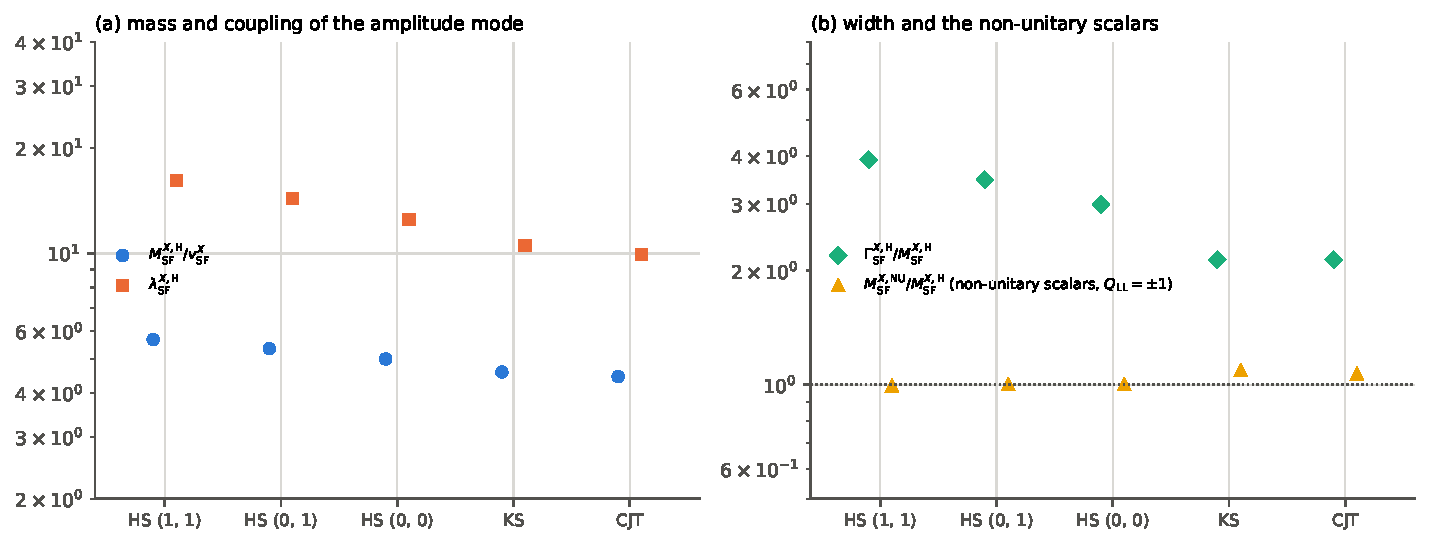
\includegraphics[width=0.85\textwidth]{fig_prd_higgs.pdf}
\caption{\label{fig:higgs}(a) $M^{X,{\rm H}}_\SF/v^X_\SF$ and $\lambda^{X,{\rm H}}_\SF$ against the Standard Model (dashed) and the
tree-level bound $8\pi/3$ of perturbative unitarity (dotted). (b) The width (\ref{eq:width}) relative to the mass, against
$\Gamma_H/m_H$ of the Standard Model, and the mass ratio of the charged non-unitary scalars to the amplitude mode.}
\end{figure*}

\paragraph*{The verdict for each method.}
Table~\ref{tab:higgs} and Fig.~\ref{fig:higgs} compare seven properties.
(1) \emph{The Higgs mechanism}: realized in every method (Sec.~\ref{sec:T0}).
(2) \emph{A neutral scalar below threshold}: in every method, at 0.82\mbox{--}0.90 of $2E^{X,{\rm gap}}_\SF$.
(3) \emph{Its mass against the scale of the breaking}: $M^{X,{\rm H}}_\SF/v^X_\SF=4.46\mbox{--}5.69$, 8.8\mbox{--}11 times the Standard-Model
value; $\lambda^{X,{\rm H}}_\SF=9.94\mbox{--}16.2$ exceeds the tree-level unitarity bound $8\pi/3=8.38$~\cite{LQT1977}; on the scale
$v^X_\SF=246.22$~GeV the amplitude mode has the mass 1.10\mbox{--}1.40~TeV.
(4) \emph{Its width}: $\Gamma^{X,{\rm H}}_\SF/M^{X,{\rm H}}_\SF=2.1\mbox{--}3.9$, a broad resonance, against $3\times10^{-5}$.
(5) \emph{No further scalars}: every method has the charged non-unitary doublet at 0.991\mbox{--}1.09 of $M^{X,{\rm H}}_\SF$.
(6) \emph{Quantum numbers}: the condensate is an isospin vector of fermion number 2 of a vector-like isospin, not a
hypercharge doublet of a chiral $SU(2)_L$; the photon is $W^3$, the $Z$ is the boson of the fermion number, and
$M^X_{W,\SF}/M^X_{Z,\SF}$ depends on two independent couplings with no custodial relation; the condensate adds a pairing gap to
the Dirac mass of the spinor field rather than generating Yukawa masses.
(7) \emph{Thermal history}: the transition lies deep in its critical region (Sec.~\ref{sec:thermal}).
In every method the superfluid realizes the Higgs mechanism and has a Higgs-like neutral scalar, but in no method can that
scalar be the observed Higgs boson. The methods differ in degree, not in kind: CJT and KS are closest, HS (1,1) farthest.

%=====================================================================================================================
\section{Is the Higgs a composite particle?}
\label{sec:composite}

In this model, yes, in every method. The field $\vec\Phi^X_\SF$ is not a field of the Lagrangian (\ref{eq:L}), whose only
matter field is the spinor field; it is the amplitude (\ref{eq:Phi}) of the pair self-energy, a composite of two spinor
charges. Its kinetic part (\ref{eq:Lkin}) has no term of its own: $Z^X_\SF$ and $Y^X_\SF$ are susceptibilities of the spinor
field. Its amplitude mode is a bound state of two quasi-particles below their threshold. This is the compositeness
condition of Bardeen, Hill and Lindner~\cite{BHL1990}: the normalization of the kinetic term of the composite field vanishes
at the cutoff, where only the spinor field exists.

The same structure explains why this composite is heavy. In Nambu-Jona-Lasinio dynamics the mass of the bound state is
tied to the gap of its constituents~\cite{NJL1961} (here $M^{X,{\rm H}}_\SF$ is 0.82\mbox{--}0.90 of $2E^{X,{\rm gap}}_\SF$), while
the scale of the breaking comes from a loop of the constituents and is small against the gap
($f^{X,{\rm I}}_\SF/E^{X,{\rm gap}}_\SF=0.16\mbox{--}0.18$). A light composite Higgs needs a cutoff far above the gap, as in top
condensation~\cite{BHL1990,HillSimmons2003}, or another mechanism, such as a pseudo-Goldstone Higgs~\cite{KaplanGeorgi1984,Agashe2005}.
Whether the Higgs boson of nature is composite is not decided here: its couplings agree with the Standard Model to several
per cent~\cite{ATLAS2022,CMS2022}, which constrains, but does not exclude, compositeness at a higher scale. What the
computation shows is that the composite Higgs of the mean-field methods of this model is not that boson.

%=====================================================================================================================
\section{Toward the gravitational sector}
\label{sec:gravity}

The factor $SL(2,\mathbb C)$ of GEE acts on the spinor index of $\Psi_\LL$ with the Lorentz connection $\Gamma^\LL_p$ of
(\ref{eq:cov}), which on the flat M31 of this paper is a pure gauge. Lord~\cite{Lord1971} considered the group of changes of
representation of the two-component spinor algebra, under which the free field equations of particles of any spin are
invariant, and made it a gauge group in the sense of Yang and Mills. Gauge invariance and Lorentz covariance require
auxiliary fields; Lord interpreted them as the potentials of a spin-two field, which is then self-interacting, and showed
that the Bargmann-Wigner equations of the linear spin-two field, modified by this self-interaction, give a nonlinear theory
identical with Einstein's; the auxiliary fields become, in addition, the gauge field of the general coordinate
transformations, the components of the affine connection. This construction is the natural route for the present model
because its spinor charges come with $SL(2,\mathbb C)$ from the super-loop~\cite{Nash2026}: the program is (i) to replace the
pure-gauge $\Gamma^\LL_p$ by Lord's gauge field and its auxiliary fields, (ii) to couple the spinor field and its pairs to
it, and (iii) to obtain the gravitational field equations with the energy-momentum tensor of the spinor field as their
source. Gauging the local Lorentz group is also the route of Utiyama and Kibble~\cite{Utiyama1956,Kibble1961,Hehl1976}.

Two consequences of the present results are already clear. First, the superfluid is a Lorentz scalar and leaves
$SL(2,\mathbb C)$ unbroken, so the condensation does not give the gravitational field a mass. Second, the condensate lowers
the energy density of the vacuum by the depth of the effective potential, $2.4\times10^{-4}\,\Lambda_\LL^4$ in CJT, that is about
$(227\ {\rm GeV})^4$ on the scale of Table~\ref{tab:higgs}, against the observed dark-energy density of about
$2.5\times10^{-47}\,{\rm GeV}^4$~\cite{PDG2024}: the cosmological-constant problem~\cite{Weinberg1989} appears here in its usual
form. The quantization of the gravitational sector, and with it the ``quantum gravity'' of the title, is beyond this paper.
A related observation, also left to future work, is that the Einstein term itself may be induced by the loop of the spinor
field~\cite{Sakharov1967,Visser2002}, just as the kinetic term (\ref{eq:Lkin}) of the composite field is.

%=====================================================================================================================
\section{Conclusions}
\label{sec:conclusions}

A spin-zero superfluid of the spinor charges of the Lorentz super-loop, solved in five mean-field methods, realizes the
Higgs mechanism of the gauge group $SL(2,\mathbb C)\times SU(2)_{\rm v}\times U(1)^{\rm F}$: massive $W^\pm$ and $Z$, a massless
photon that does not mix with the boson of the fermion number, the surviving group $SL(2,\mathbb C)\times O(2)$ with the $U(1)$
of the electric charge, and a composite amplitude mode below the threshold of two quasi-particles. Its Higgs field is
composite by construction. Quantitatively it is not the Standard-Model Higgs sector: the amplitude mode is 8.8\mbox{--}11
times too heavy against the scale of the breaking, broad and strongly coupled, there are charged scalars of comparable
mass, and the thermal transition lies inside a critical region of width ${\rm Gi}\approx7.6\mbox{--}11$, so that its
mean-field description is not reliable. The gravitational sector will be added through Lord's gauge theory of the local
change of spinor representation, for which the model already has the place.

%=====================================================================================================================
\section*{Data availability}

The data that support the findings of this article are openly available in the repository of PROJECT
spacetimes~\cite{Repo}, folder \texttt{Revision\_HS\_CJT\_and\_Kohn-Sham}: the data files (\texttt{data/}), the Rust and Python
programs that produce them (\texttt{rust/}, \texttt{python/}), the reports of their checks, the Wolfram Language notebook, and
the scripts that build this article from the data (\texttt{paper\_prd/}). The Supplemental Material~\cite{SM} lists the files
with their SHA-256 checksums.

\begin{acknowledgments}
The computations used the SUNDIALS integrators in a Rust implementation, numpy and LAPACK.
\end{acknowledgments}

\bibliography{references}

\end{document}
